%----------------------------Meta Data----------------------------%
\documentclass{beamer}

%Packages
\usepackage{pgfpages}
\usepackage{tikz}
\usepackage{lcg}

\usetheme{Frankfurt}

\setbeamertemplate{navigation symbols}{} % Turn off navigation symbols.
\graphicspath{{Figures/}}

%Presentation Specific
\title{How Many Guards in the Gallery?}
%\subtitle{Optional Subtitle}
\author{Marvin Buff}
\institute{University of Basel}
\date{Recreational Science, 2017}

%Adds the navigation before every new section.
\AtBeginSection[]
{
  \begin{frame}
    \frametitle{Table of Contents}
    \tableofcontents[currentsection]
  \end{frame}
}


%----------------------------Begin Document----------------------------%
\begin{document}

%-------------Frame::Title---------------%
\begin{frame}
  \titlepage
\end{frame}

%-------------Frame::Content---------------%
\begin{frame}{Outline}
  \tableofcontents%[pausesections]
\end{frame}


%-------------Section::One-----------------%
\section{First Section}
\subsection{First Subsection}%This add bullet on navigation

%-------------Frame::Graphic---------------%
\begin{frame}{Setting}
    \begin{block}{Include Graphic}
        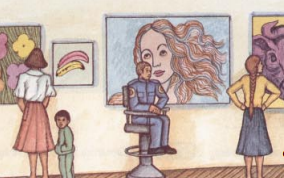
\includegraphics[width=1\textwidth]{guard} 
    \end{block}   
\end{frame}

\subsection{Second Subsection}

%-------------Frame::Tikz-----------------%
\begin{frame}{Split Columns}
    \begin{columns}
    \begin{column}{0.5\textwidth}
          \begin{block}{A normal block}
              \begin{tikzpicture}[scale=2.6]
                    \foreach \x in {0,60,...,300} {
                        \draw[fill] (\x:1 cm) -- (\x + 60:1 cm);
                        }
                    \draw[fill] (0,0) circle (1pt);
              \end{tikzpicture}
          \end{block} 
    \end{column}
    \begin{column}{0.5\textwidth}  %%<--- here
        \begin{exampleblock}{Example block}
            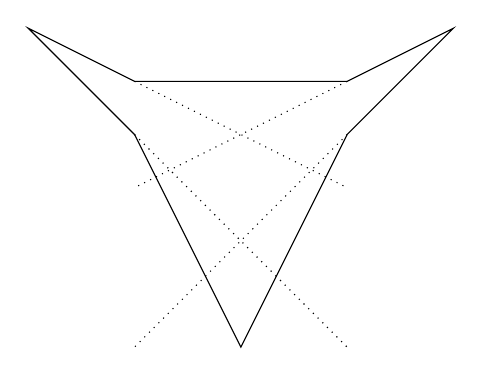
\begin{tikzpicture}[scale=1.35]
                    \draw[draw] (4,4) -- (3,3.5) -- (1,3.5) -- (0,4) 
                                -- (1,3) -- (2,1) -- (3,3) -- cycle;
                    \draw[dotted] (1,3.5) -- (3,2.5);
                    \draw[dotted] (3,3) -- (1,1);
                    \draw[dotted] (1,3) -- (3,1);
                    \draw[dotted] (3,3.5) -- (1,2.5);
            \end{tikzpicture}
        \end{exampleblock} 
    \end{column}
    \end{columns}
\end{frame}

%-------------Section::Two-----------------%
\section{Second Section}
\subsection*{Hidden Section}%Bullet point, but not in navigation

%-------------Frame::Proof-----------------%
\begin{frame}{Some Proof}
  \begin{theorem}
      $g(n) \leq \lfloor n/3\rfloor$
  \end{theorem}
  \begin{block}{Proof Sketch}
      \begin{enumerate}
      \item Every simple polygon can be guarded 
            with at most $\lfloor n/3\rfloor$ vertex guards.
      \item Some simple polygons require at least $\lfloor n/3\rfloor$ guards.
      \end{enumerate}
  \end{block}
\end{frame}

%-------------Section::Summary-------------%
\section*{Summary}
\subsection*{Summary}
\begin{frame}{Summary}
\begin{block}{Take Home Message}
  \begin{itemize}
      \vskip5pt
      \item \color{blue}The Art Gallery Problem \vskip5pt
      \item Fisk's Proof:  $g(n) \leq \lfloor n/3\rfloor$ \vskip5pt
      \item Triangulation
      \begin{itemize}
          \item Ear Clipping $O(n^2)$
          \item Sweep Line $O(n\ log\ n)$
          \item Las Vegas $O(n\ log^*\ n)$
          \item Polygon Cutting $O(n)$
      \end{itemize} \vskip15pt
  \end{itemize}
  \end{block}
\end{frame}

%-------------Frame::Questions-------------%
\begin{frame}
    \begin{center}
        \huge Questions? \normalsize
    \end{center}
\end{frame}


%-------------Appendix---------------%
\appendix
\section<presentation>*{\appendixname}
\subsection<presentation>*{For Further Reading}

\begin{frame}[allowframebreaks]
  \frametitle<presentation>{For Further Reading}
    
  \begin{thebibliography}{10}
    
  \beamertemplatebookbibitems
  % Start with overview books.
    
  \beamertemplatearticlebibitems
  % Followed by interesting articles. Keep the list short. 

  \bibitem{stewart1994}
    I. Stewart.
    \newblock How Many Guards in the Gallery?
    \newblock {\em Scientific American 270}, no. 5 (1994): 118-20. 
  \end{thebibliography}
\end{frame}

\begin{frame}
    \begin{block}{Some equation}
        \begin{equation}
            \textsf{log}^*\ n=\left\{
                \begin{array}{ll}
                  0 & \textsf{if }n \leq 1\\
                  1 + \textsf{log}^*~(\textsf{log }n) & \textsf{if } n > 1
                \end{array}
              \right.
        \end{equation}
    \end{block}
\end{frame}

\end{document}




